\documentclass[letterpaper,11pt]{article}
\oddsidemargin -1.0cm \textwidth 17.5cm

\usepackage[utf8]{inputenc}
\usepackage[activeacute,spanish]{babel}
\usepackage{amsfonts,setspace}
\usepackage{amsmath}
\usepackage{amssymb, amsmath, amsthm}
\usepackage{comment}
\usepackage{amssymb}
\usepackage{dsfont}
\usepackage{anysize}
\usepackage{multicol}
\usepackage{enumerate}
\usepackage{graphicx}
\usepackage[left=1.5cm,top=2cm,right=1.5cm, bottom=1.7cm]{geometry}
\setlength\headheight{1.5em} 
\usepackage{fancyhdr}
\usepackage{multicol}
\usepackage{hyperref}
\usepackage{wrapfig}
\pagestyle{fancy}
\fancyhf{}
\renewcommand{\labelenumi}{\normalsize\bfseries P\arabic{enumi}.}
\renewcommand{\labelenumii}{\normalsize\bfseries (\alph{enumii})}
\renewcommand{\labelenumiii}{\normalsize\bfseries \roman{enumiii})}

\begin{document}

\fancyhead[L]{\itshape{Facultad de Ciencias F\'isicas y Matem\'aticas}}
\fancyhead[R]{\itshape{Universidad de Chile}}

\begin{minipage}{11.5cm}
    \begin{flushleft}
        \hspace*{-0.6cm}\textbf{FI1000-5 Introducción a la Física Clásica}\\
        \hspace*{-0.6cm}\textbf{Profesora:} Paulina Lira\\
        \hspace*{-0.6cm}\textbf{Auxiliares:} Alejandro Silva, Felipe Kaschel, Juan Cristóbal Castro\\
    \end{flushleft}
\end{minipage}

\begin{picture}(2,3)
    \put(366,-4){
\includegraphics[scale=0.9]{2020-1/Imágenes/logo/dfi-fcfm.pdf}}
\end{picture}

\begin{center}
	\LARGE \bf Auxiliar \# 12   \\
\end{center}

\vspace{-1cm}
\begin{enumerate}\setlength{\itemsep}{0.4cm}

\rfoot[]{pág. \thepage}

\item[]

\item Una persona se encuentra sobre una plataforma móvil, tal que sus masas suman $M$, sobre la plataforma lleva consigo dos ladrillos de masa $m$. Si la plataforma está inicialmente en reposo y en un instante la persona lanza horizontalmente uno de los ladrillos y luego otro hacia atrás de la plataforma, con una velocidad $v_o= 2 m/s$ respecto a él mismo. ¿Que velocidad $v$ adquirirá la plataforma?


\item En la figura se  muestra un bloque de masa $M$, amarrado al techo mediante un resorte ideal y posado sobre una superficie horizontal resbaladiza. El resorte es de constante elástica $k$ y largo natural $L$. En el esquema el resorte está vertical y sin elongación. Una bala de masa $m$ es disparada horizontalmente y se incrusta en el bloque (choque perfectamente inelástico).
\begin{enumerate}
    \item Determine la rapidez máxima de la bala a fin de que el bloque nunca pierda contacto con la superficie.
    \item Describa como será el movimiento subsecuente.
\end{enumerate}

\begin{figure}[h!]
    \centering
    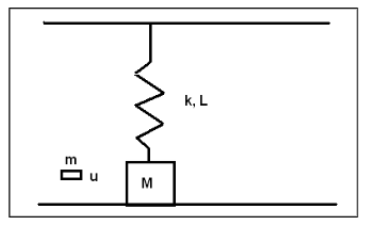
\includegraphics[scale=0.8]{2020-1/Imágenes/Aux12/p1a12.png}
\end{figure}

\item Una partícula colisiona a una segunda partícula de igual masa que estaba inicialmente en reposo. Si colisionan elásticamente sobre un plano horizontal libre de roce, determine el angulo $\phi$ de salida de la particula inicialmente en reposo si la primera partícula se desvía un ándulo $\theta$ con respecto a la dirección que traía antes de la colisión.

\begin{figure}[h!]
    \centering
    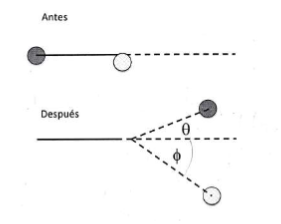
\includegraphics[scale=1]{2020-1/Imágenes/Aux12/p2a12.png}
\end{figure}



\end{enumerate}
\end{document}